%% ****** Start of file apstemplate.tex ****** %
%%
%%
%%   This file is part of the APS files in the REVTeX 4 distribution.
%%   Version 4.1r of REVTeX, August 2010
%%
%%
%%   Copyright (c) 2001, 2009, 2010 The American Physical Society.
%%
%%   See the REVTeX 4 README file for restrictions and more information.
%%
%
% This is a template for producing manuscripts for use with REVTEX 4.0
% Copy this file to another name and then work on that file.
% That way, you always have this original template file to use.
%
% Group addresses by affiliation; use superscriptaddress for long
% author lists, or if there are many overlapping affiliations.
% For Phys. Rev. appearance, change preprint to twocolumn.
% Choose pra, prb, prc, prd, pre, prl, prstab, prstper, or rmp for journal
%  Add 'draft' option to mark overfull boxes with black boxes
%  Add 'showpacs' option to make PACS codes appear
%  Add 'showkeys' option to make keywords appear

\documentclass[aps,pre,preprint,groupedaddress, floatfix]{revtex4-1}
%\documentclass[aps,prl,preprint,superscriptaddress]{revtex4-1}
%\documentclass[aps,prl,reprint,groupedaddress]{revtex4-1}

\input ../inputs/setupSveZha
\input ../inputs/editsDasbuch   %% editing comments, DasBuch style
\input ../inputs/def            %% do not edit; update from dasbuch/book/inputs/def.tex
\input ../inputs/defsSveZha     %% all diffusion project edits: \renewcommand, etc


% You should use BibTeX and apsrev.bst for references
% Choosing a journal automatically selects the correct APS
% BibTeX style file (bst file), so only uncomment the line
% below if necessary.
%\bibliographystyle{apsrev4-1}

\begin{document}

% Use the \preprint command to place your local institutional report
% number in the upper righthand corner of the title page in preprint mode.
% Multiple \preprint commands are allowed.
% Use the 'preprintnumbers' class option to override journal defaults
% to display numbers if necessary
%\preprint{}

%Title of paper
\title{Diffuse globally, compute locally: a cyclist tale}

% repeat the \author .. \affiliation  etc. as needed
% \email, \thanks, \homepage, \altaffiliation all apply to the current
% author. Explanatory text should go in the []'s, actual e-mail
% address or url should go in the {}'s for \email and \homepage.
% Please use the appropriate macro foreach each type of information

% \affiliation command applies to all authors since the last
% \affiliation command. The \affiliation command should follow the
% other information
% \affiliation can be followed by \email, \homepage, \thanks as well.
\author{Tingnan Zhang, Daniel I. Goldman and Predrag Cvitanovi\'c}
\email[corresponding to: ]{predrag@gatech.edu}
%\homepage[]{Your web page}
%\thanks{}
%\altaffiliation{}
\affiliation{School of Physics, Georgia Institute of Technology}

%Collaboration name if desired (requires use of superscriptaddress
%option in \documentclass). \noaffiliation is required (may also be
%used with the \author command).
%\collaboration can be followed by \email, \homepage, \thanks as well.
%\collaboration{}
%\noaffiliation

\date{\today}

\begin{abstract}
\input abstract
\end{abstract}

% insert suggested PACS numbers in braces on next line
\pacs{}
% insert suggested keywords - APS authors don't need to do this
%\keywords{}

%\maketitle must follow title, authors, abstract, \pacs, and \keywords
\maketitle

% body of paper here - Use proper section commands
% References should be done using the \cite, \ref, and \label commands

\section{Introduction}

\input intro

\section{Diffusion confusion}

\subsection{Translational Symmetry}

\begin{figure}
\begin{center}
(a)\includegraphics[width=0.29\textwidth]{diskDirectionsElCell}
(b)\includegraphics[width=0.29\textwidth]{diskDirecsElCell05}
(c)\includegraphics[width=0.29\textwidth]{diskDirecsElCell05red}
\end{center}
\caption{
Elementary cell symbolic dynamics is obtained by labeling the translation
vectors connecting the center of the current disk to the center of the
next disk.
(a) The finite horizon is here imposed by limiting jumps from the
center cell to only the short jumps (six even labels $0, 2,\cdots,10$)
and the `long jumps' (six odd labels $1, 3,\cdots,11$).
(b) Running mode \cycle{05} advances by $\hn_4$ per period.
(c) In the elementary cell this is a \po\ \cycle{05}
    of topological length 2.
    }
\label{diskDirectionsElCell}
\end{figure}

\subsection{Into fundamental domain}
\begin{figure}[htbp]
\begin{center}
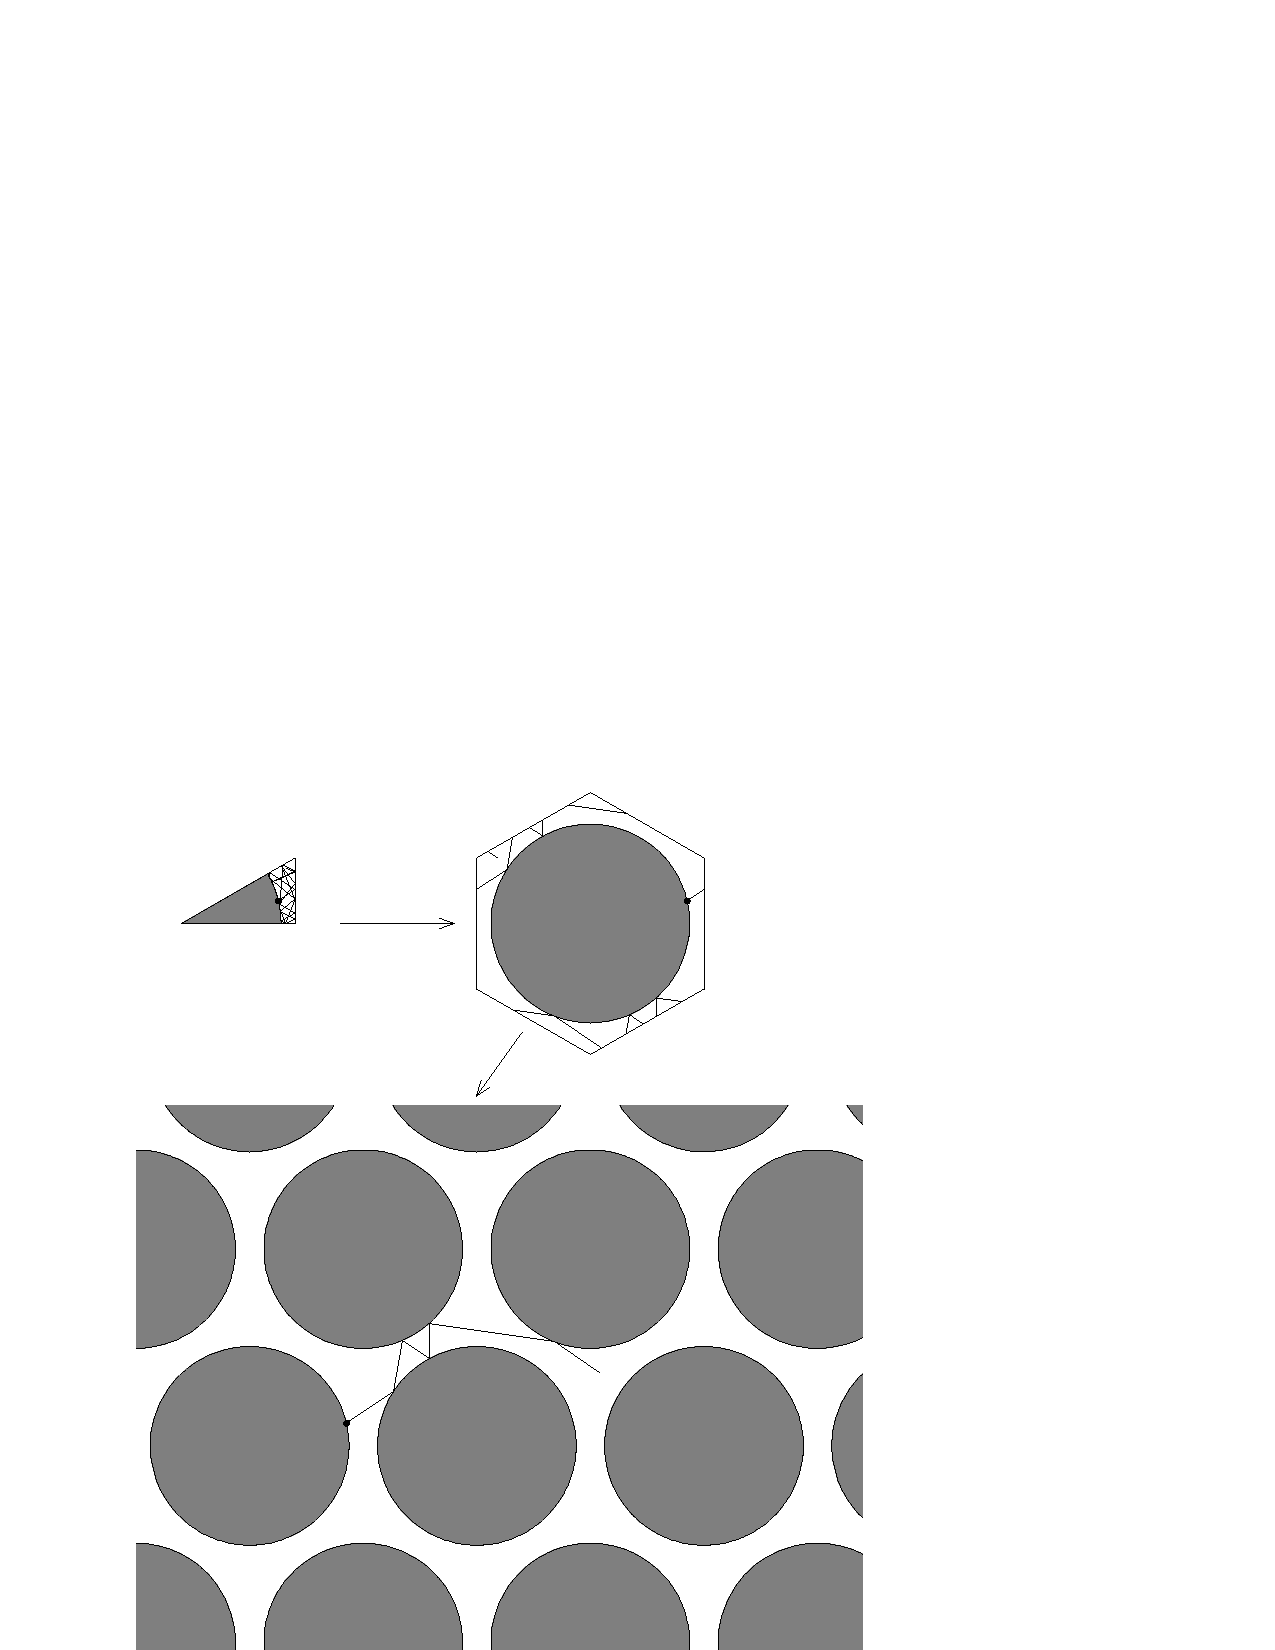
\includegraphics[width=0.45\textwidth]{schreiberFig1}
\end{center}
\caption[]{\label{fig:schrieberFig1}}
Motion in fundamental domain (FD), elementary cell (EC) and full space.
\end{figure}

\begin{figure}[htbp]
\begin{center}
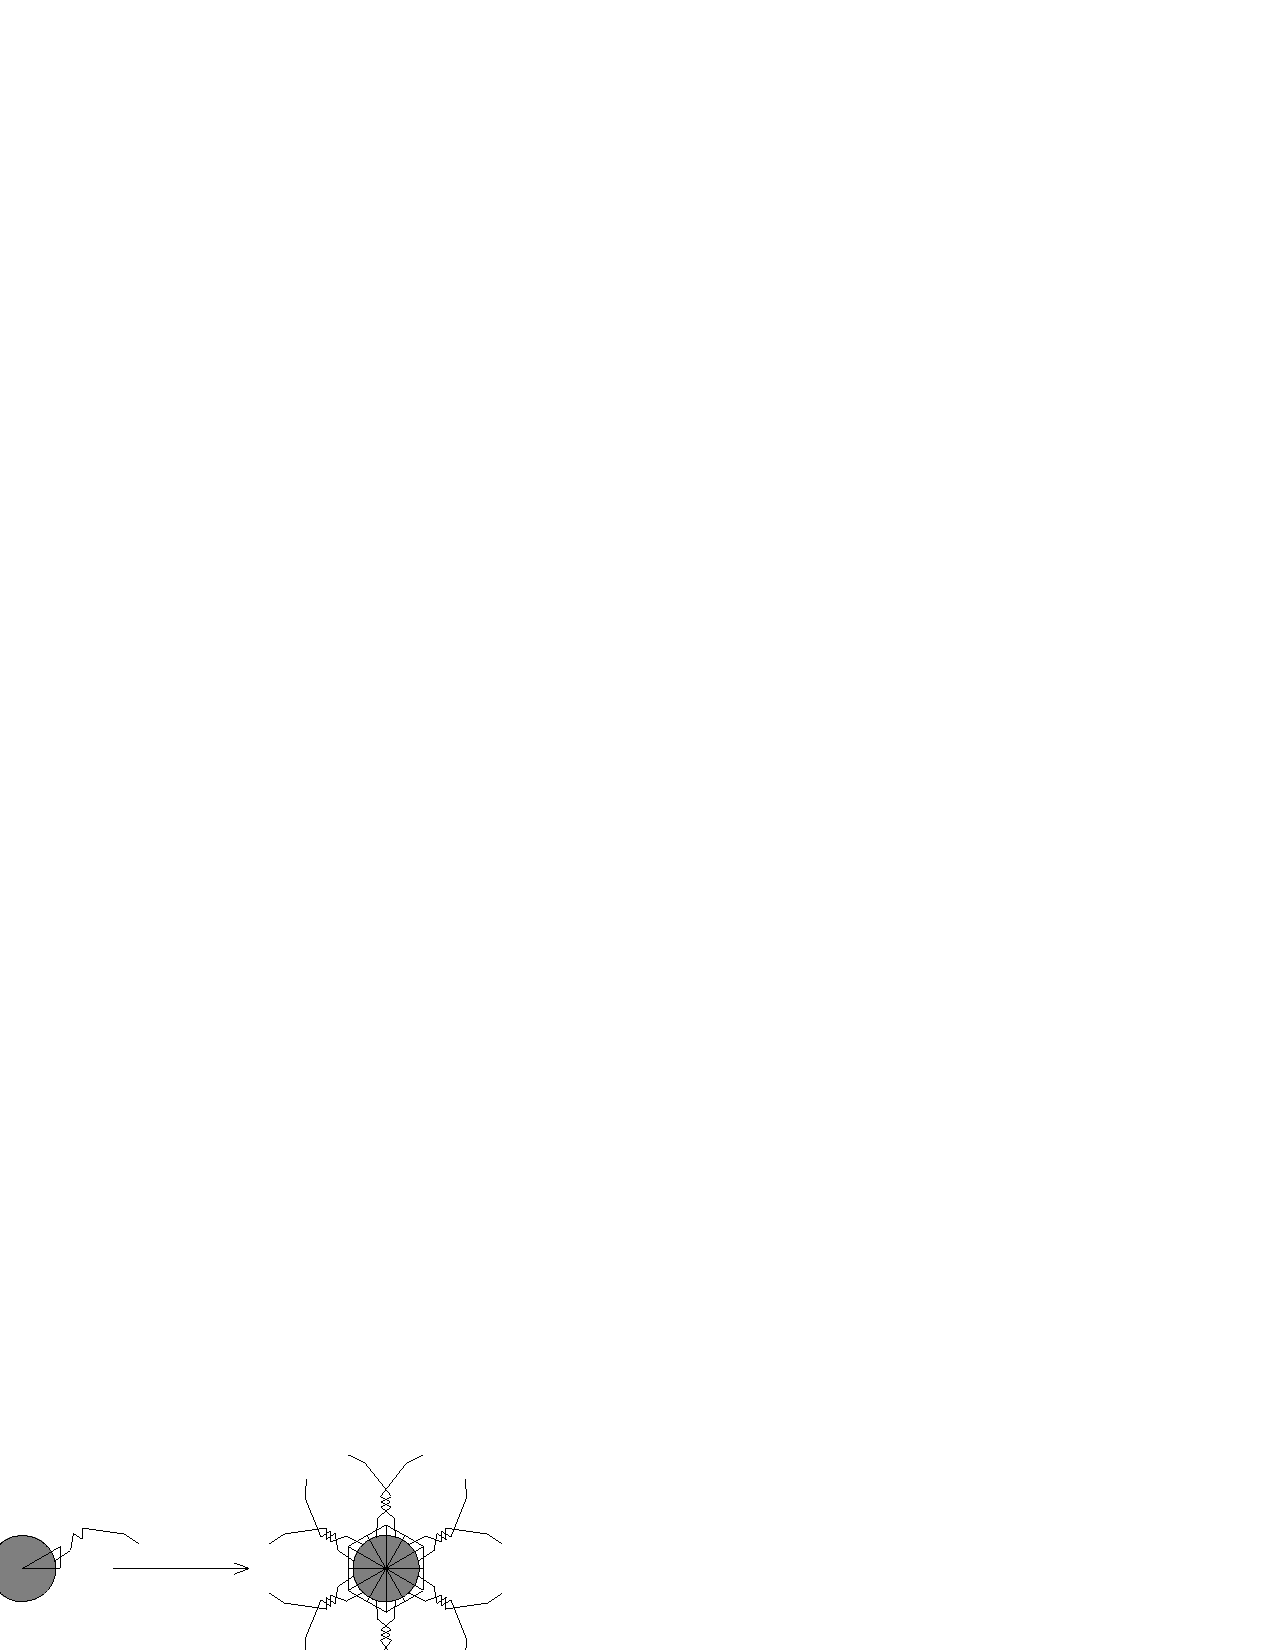
\includegraphics[width=0.45\textwidth]{schreiberFig2}
\end{center}
\caption[]{ \label{fig:schrieberFig2}
An (unwrapped) trajectory (in full space) and its 12 copies after
applying point group actions to it.}
\end{figure}

\begin{figure}[htbp]
\begin{center}
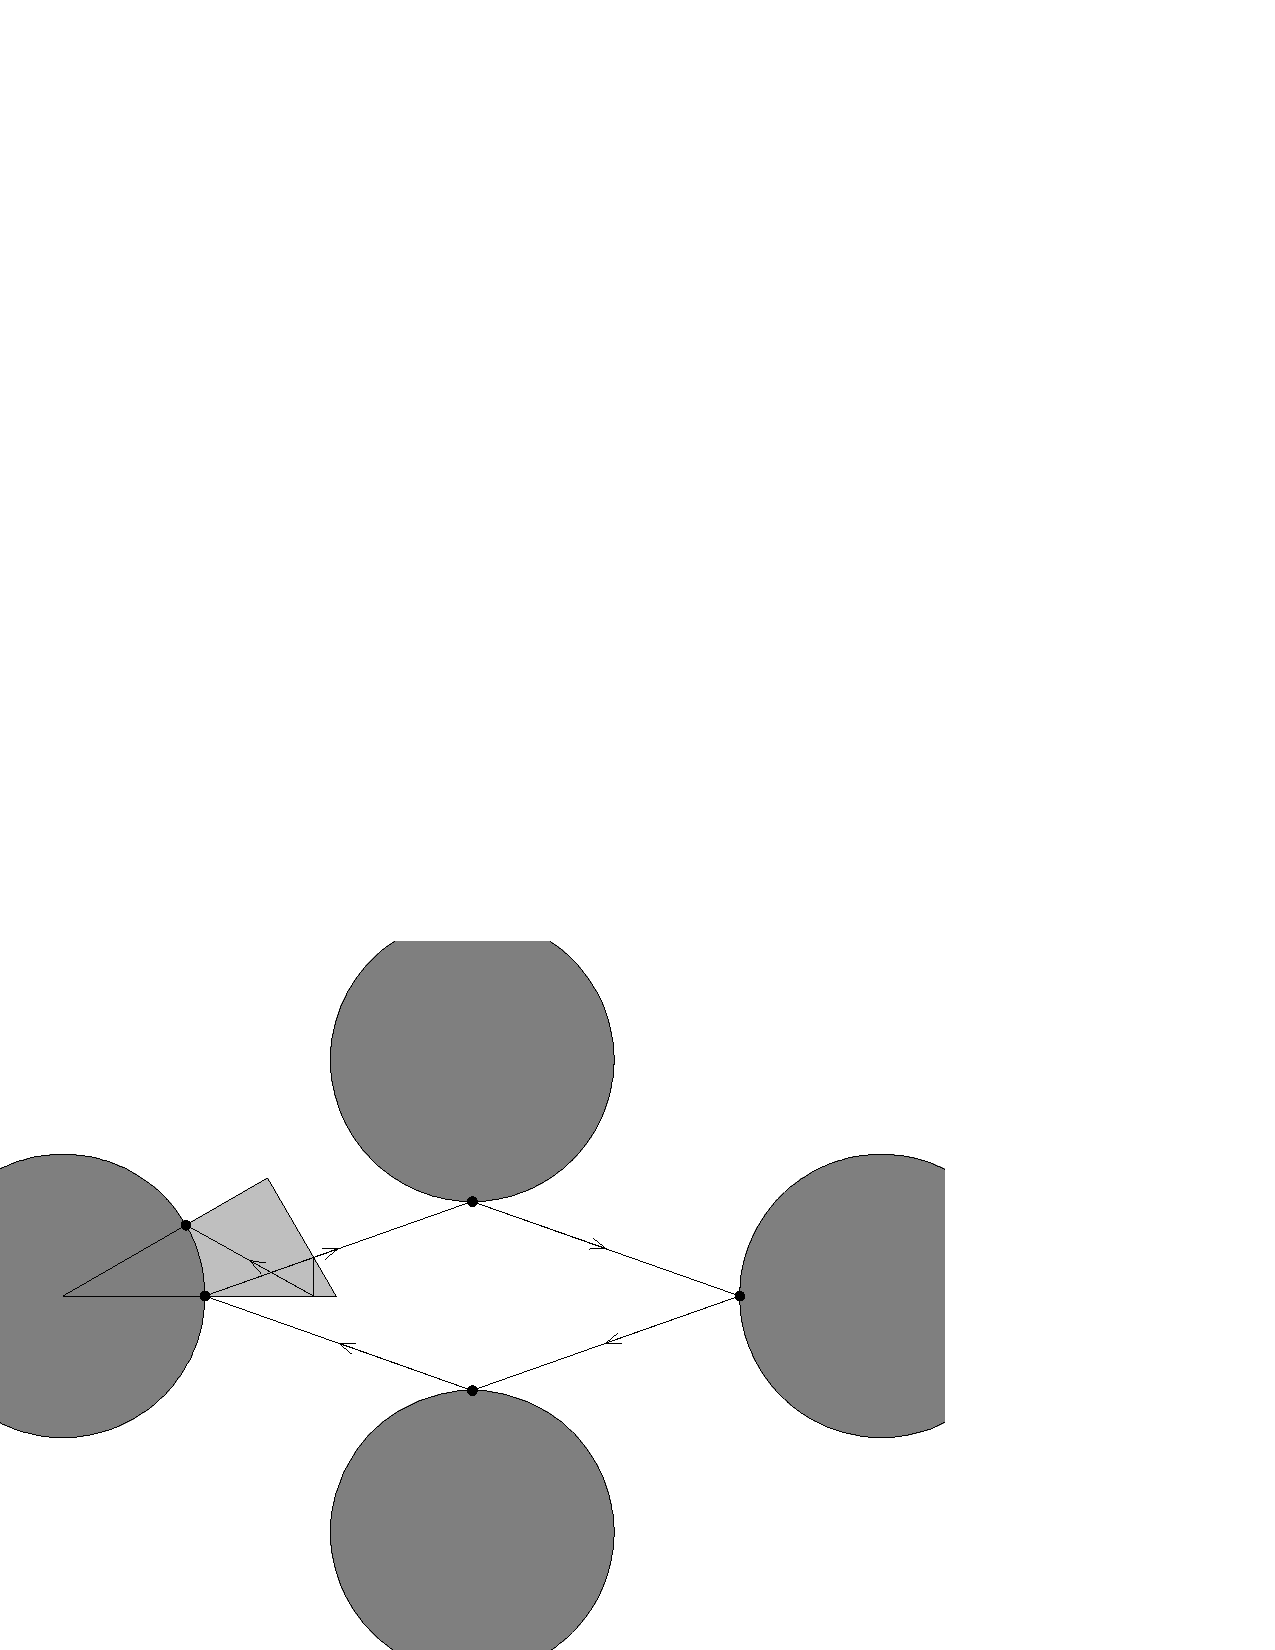
\includegraphics[width=0.45\textwidth]{schreiberFig3}
\caption[]{Multiplicity of periodic orbits in FD. \label{fig:schrieberFig3}}
\end{center}

\end{figure}
\subsubsection{Grammar of FD cycle}
\begin{figure}
\begin{center}
(a) 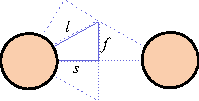
\includegraphics[width=0.45\textwidth]{7diskFundDflips}
(b) 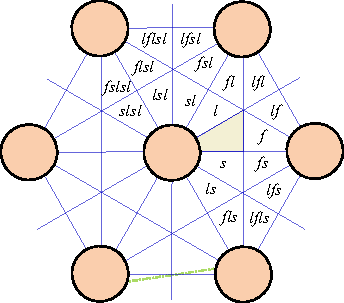
\includegraphics[width=0.45\textwidth]{7diskFundDtiles}
\end{center}
\caption{\label{fig:7diskFundDflips}
(a) The three generators of tiling of the plane by a fundamental domain:
two generators of \Dn{12} tiling, reflection $s$ across the short
disk-disk separation, reflection  $\ell$  across the long disk-disk
separation;
and
a translation generator $f$ that pivots (`flips') a disk center to disk
center by flip across the symmetry line normal to the short disk-disk
separation.
(5) Tiling of the 7-disk by copies of the fundamental domain, labelled
by a (not unique) sequence of the three generators
$\{s,\ell,f\}$, chosen so that each sequence contain one and only on
    disk-to-disk pivot $f$.
}
\end{figure}

\begin{figure}[htbp]
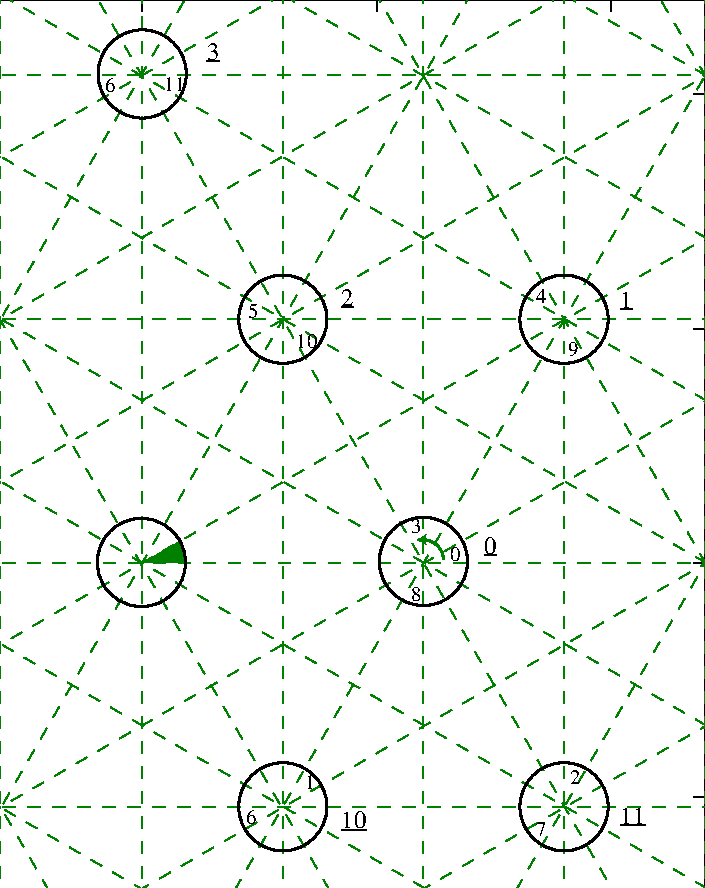
\includegraphics[width=0.45\textwidth]{fdSymbolIllustration}
\caption{\label{fig:fdflights}
Topologically distinct flights, with imposed finite horizon.
}
\end{figure}

\subsubsection{How point group changes translation}
Starting from each point on the cycle, the translation in full space is
different after completion of one cycle.


\subsubsection{Gymnastics of equations}

\Group-equivariance of the displacement in the full space.

\begin{align}
\tr{\cal L}^t &=
\sum_{\alpha \in\II_G} \tr{\cal L}_{\alpha}^t\nonumber\\
\tr{\cal L}_{\alpha}^t &=
\frac{d_\alpha}{|G|}\sum_{\sigma \in G}\sum_{h\in G}\chi_\alpha(h)
\int_{\t {\cal M}} d\tx \delta (h\tx - f^t(\tx))
e^{\beta\cdot\sigma\cdot\hphi^t(\tx)}~,
\label{e1}
\end{align}

\begin{align}
\frac{1}{\zeta_{\alpha}(\beta,s,z)} &=\exp\left(
-\frac{d_\alpha}{|G|}\sum_{\sigma\in G}\sum_{\tp}\frac{1}{n_{\tp}}
\sum_{\tx_{i}\in\tilde{p}}\sum_{r=1}^{\infty}
\frac{t_{\tp}^{r}}{r}\chi_{\alpha}(\hp^{r}(\tx_i))
e^{\beta\cdot\sigma\cdot\hat{L}_{\tp}(r,\tx_i)}
\right)
\end{align}
where we have defined
\begin{equation}
t_{\tp}\equiv \frac{z^{n_{\tp}}e^{-sT_{\tp}}}{|\ExpaEig_\tp|}
\end{equation}
and
\begin{equation}
\hat{L}_{\tp}(r,\tx_i)\equiv (e+\hp^{-1}(\tx_i)\cdots+\hp^{-r+1}(\tx_i))\cdot\hn_{\tp}(\tx_i)
\end{equation}

We are interested in the one dimensional, symmetric trivial
representation with $ d_\alpha = 1 $ and all $ \chi(h) = 1 $,; there by
we drop the subscript $ \alpha $ in the following calculation. Partial
derivative with respect to $\beta$:
\begin{align}
\frac{\partial^{2}}{\partial\beta^{2}}\frac{1}{\zeta(\beta,s,z)}
 &=\frac{1}{\zeta(\beta,s,z)}\left(\left(\frac{1}{|G|}
\sum_{\sigma\in G}\sum_{\tp}\sum_{\tx_i\in \tp}\sum_{r=1}^{\infty}\frac{\sigma\cdot \hat{L}_{\tp}(r,\tx_i)t_{\tp}^r e^{\beta\cdot\sigma\cdot \hat{L}_{\tp}(r,\tx_i)}}{n_{\tp}r}\right)^{2}\right.\nonumber\\
 & \left.-\frac{1}{|G|}\sum_{\sigma\in G}\left(\sum_{\tp}\sum_{\tx_i\in \tp}\sum_{r=1}^{\infty}\frac{\vert \sigma\cdot \hat{L}_{\tp}(r,\tx_i)\vert^{2}t_{\tp}^{r}e^{\beta\cdot\sigma\cdot \hat{L}_{\tp}(r,\tx_i)}}{n_{p}r}\right)\right).
\end{align}
The first term in the formula corresponds to $ \langle\hx\rangle^2 $ and
second to $ \langle\hx^2\rangle $


\section{Results and Discussions}

\begin{table}[htbp]
{\small
%\begin{center}
\begin{tabular}{|r|r|r|l|l|}
\hline
$\period{p}$ & \# cycles & $\zeta$(0,0) & $\lambda$ & D \\ \hline\hline
1      & 0      &   -    &   -  &   - \\
2      & 24     & -0.31697 & 1.330 & 0.375\\
3      & 64     & -0.54152 & 1.435 & 0.339\\
4      & 168    & -0.09764 & 1.902 & 0.284\\
5      & 516    &  0.02334 & 2.324 & 0.215\\
6      & 1589   & -0.00481 & 1.975 & 0.133\\
7      & 5700   & -0.01241 & 1.885 & 0.184\\
8      & 20729  & -0.01006 & 1.785 & 0.247\\ \hline\hline
\multicolumn{4}{|l|}{numerical experiment} 1.760 & 0.25 \\ \hline
\end{tabular}
\hfill
\begin{tabular}{|r|r|r|l|l|}
\hline
$\period{p}$ & \# cycles & $\zeta$(0,0) & $\lambda$ & D \\ \hline\hline
1      & 5      &   -0.2169759    &   1.39193  &   0.37795 \\
2      & 10     & -0.0248233 & 1.74541 & 0.23118\\
3      & 33     & -0.0221962 & 1.72235 & 0.25257\\
4      & 108    & -0.0002192 & 1.74450 & 0.24165\\
5      & 373    &  0.0023463 & 1.76079 & 0.24468\\
6      & 1378   &  0.0096330 & 1.75610 & 0.24068\\ \hline\hline
\multicolumn{3}{|l|}{numerical experiment}
                           & 1.760 & 0.25
\\ \hline
\end{tabular}
}

\caption{\label{TCELL2}
Results for $w$=0.3. (left) Schreiber 1992 calculation\rf{CGS92} (and
this paper) in EC. (right) Our calculation in FD. Gaspard 1992
note: ``My numerical estimate for the Lyapunov exponent when $w=0.3$ is
$\lambda = 1.760 \pm 0.002$, which supports the result of this table.''
}
\end{table}

\begin{figure}
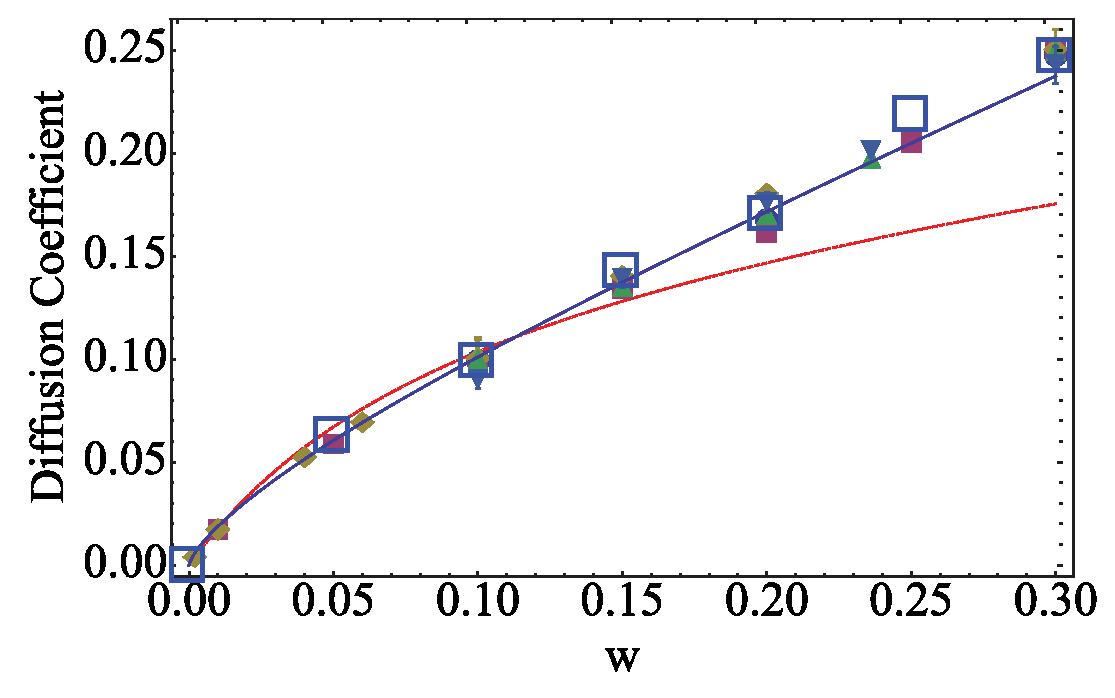
\includegraphics[width=0.5\textwidth]{diffcoefplot}
\caption[]{\label{fig:results}
Diffusion coefficients as a function of inter-disk separation distance
$w$.
          }
\end{figure}
% Put \label in argument of \section for cross-referencing
%\section{\label{}}

% If in two-column mode, this environment will change to single-column
% format so that long equations can be displayed. Use
% sparingly.
%\begin{widetext}
% put long equation here
%\end{widetext}

% figures should be put into the text as floats.
% Use the graphics or graphicx packages (distributed with LaTeX2e)
% and the \includegraphics macro defined in those packages.
% See the LaTeX Graphics Companion by Michel Goosens, Sebastian Rahtz,
% and Frank Mittelbach for instance.
%
% Here is an example of the general form of a figure:
% Fill in the caption in the braces of the \caption{} command. Put the label
% that you will use with \ref{} command in the braces of the \label{} command.
% Use the figure* environment if the figure should span across the
% entire page. There is no need to do explicit centering.

% \begin{figure}
% \includegraphics{}%
% \caption{\label{}}
% \end{figure}

% Surround figure environment with turnpage environment for landscape
% figure
% \begin{turnpage}
% \begin{figure}
% \includegraphics{}%
% \caption{\label{}}
% \end{figure}
% \end{turnpage}

% tables should appear as floats within the text
%
% Here is an example of the general form of a table:
% Fill in the caption in the braces of the \caption{} command. Put the label
% that you will use with \ref{} command in the braces of the \label{} command.
% Insert the column specifiers (l, r, c, d, etc.) in the empty braces of the
% \begin{tabular}{} command.
% The ruledtabular enviroment adds doubled rules to table and sets a
% reasonable default table settings.
% Use the table* environment to get a full-width table in two-column
% Add \usepackage{longtable} and the longtable (or longtable*}
% environment for nicely formatted long tables. Or use the the [H]
% placement option to break a long table (with less control than
% in longtable).
% \begin{table}%[H] add [H] placement to break table across pages
% \caption{\label{}}
% \begin{ruledtabular}
% \begin{tabular}{}
% Lines of table here ending with \\
% \end{tabular}
% \end{ruledtabular}
% \end{table}

% Surround table environment with turnpage environment for landscape
% table
% \begin{turnpage}
% \begin{table}
% \caption{\label{}}
% \begin{ruledtabular}
% \begin{tabular}{}
% \end{tabular}
% \end{ruledtabular}
% \end{table}
% \end{turnpage}

% Specify following sections are appendices. Use \appendix* if there
% only one appendix.
%\appendix
%\section{}

% If you have acknowledgments, this puts in the proper section head.
%\begin{acknowledgments}
% put your acknowledgments here.
%\end{acknowledgments}

Test of the temporary diffuse specific bibliography - \refref{RoMo08a}
is a repeat, for testing purpose only.
% Create the reference section using BibTeX:
\bibliography{../bibtex/siminos,../bibtex/diffuse}

\PublicPrivate{}{% switch \PublicPrivate{
\input ../tingnan/flotsam
      }% end \PublicPrivate{


\end{document}
%
% ****** End of file apstemplate.tex ******
